\documentclass[tikz,border=6pt]{standalone}
\usepackage{amsmath,bm}
\usetikzlibrary{arrows.meta,positioning,fit}

\begin{document}
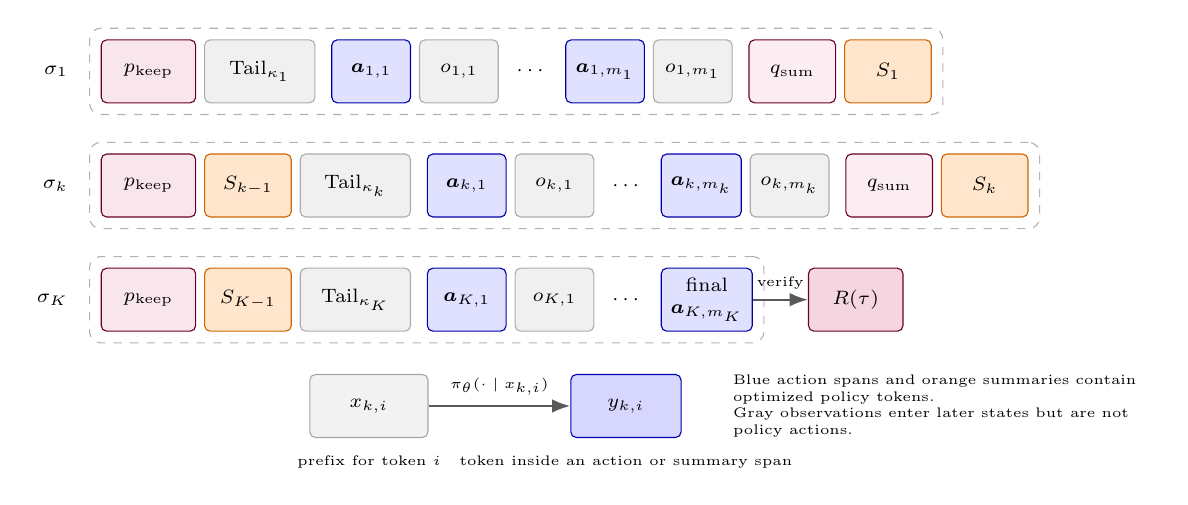
\begin{tikzpicture}[
  font=\scriptsize,
  >=Latex,
  flow/.style={->, thick, draw=gray!70!black},
  retained/.style={
    rounded corners=2pt,
    draw=purple!55!black,
    fill=purple!10,
    minimum width=12mm,
    minimum height=8mm,
    align=center
  },
  action/.style={
    rounded corners=2pt,
    draw=blue!65!black,
    fill=blue!12,
    minimum width=10mm,
    minimum height=8mm,
    align=center
  },
  observation/.style={
    rounded corners=2pt,
    draw=gray!65,
    fill=gray!12,
    minimum width=10mm,
    minimum height=8mm,
    align=center
  },
  summary/.style={
    rounded corners=2pt,
    draw=orange!80!black,
    fill=orange!20,
    minimum width=11mm,
    minimum height=8mm,
    align=center
  },
  instruction/.style={
    rounded corners=2pt,
    draw=purple!55!black,
    fill=purple!7,
    minimum width=11mm,
    minimum height=8mm,
    align=center
  },
  segment/.style={
    rounded corners=4pt,
    draw=gray!60,
    dashed,
    inner sep=4pt
  },
  state/.style={
    rounded corners=2pt,
    draw=gray!70,
    fill=gray!10,
    minimum width=15mm,
    minimum height=8mm,
    align=center
  },
  token/.style={
    rounded corners=2pt,
    draw=blue!70!black,
    fill=blue!16,
    minimum width=14mm,
    minimum height=8mm,
    align=center
  },
  note/.style={font=\tiny, align=center}
]

% First context-bounded segment.
\node[anchor=east] at (-0.2,3.0) {$\sigma_1$};
\node[retained] (p1) at (0.7,3.0) {$p_{\mathrm{keep}}$};
\node[observation, right=1mm of p1, minimum width=14mm] (tail1)
  {$\operatorname{Tail}_{\kappa_1}$};
\node[action, right=2mm of tail1] (a11) {$\bm a_{1,1}$};
\node[observation, right=1mm of a11] (o11) {$o_{1,1}$};
\node[right=1mm of o11] (d11) {$\cdots$};
\node[action, right=1mm of d11] (a1m) {$\bm a_{1,m_1}$};
\node[observation, right=1mm of a1m] (o1m) {$o_{1,m_1}$};
\node[instruction, right=2mm of o1m] (q1) {$q_{\mathrm{sum}}$};
\node[summary, right=1mm of q1] (S1) {$S_1$};
\node[segment, fit=(p1)(S1)] {};

% A middle segment, reconstructed from the preceding summary and optional tail.
\node[anchor=east] at (-0.2,1.55) {$\sigma_k$};
\node[retained] (pk) at (0.7,1.55) {$p_{\mathrm{keep}}$};
\node[summary, right=1mm of pk] (Skm1) {$S_{k-1}$};
\node[observation, right=1mm of Skm1, minimum width=14mm] (tailk)
  {$\operatorname{Tail}_{\kappa_k}$};
\node[action, right=2mm of tailk] (ak1) {$\bm a_{k,1}$};
\node[observation, right=1mm of ak1] (ok1) {$o_{k,1}$};
\node[right=1mm of ok1] (dk1) {$\cdots$};
\node[action, right=1mm of dk1] (akm) {$\bm a_{k,m_k}$};
\node[observation, right=1mm of akm] (okm) {$o_{k,m_k}$};
\node[instruction, right=2mm of okm] (qk) {$q_{\mathrm{sum}}$};
\node[summary, right=1mm of qk] (Sk) {$S_k$};
\node[segment, fit=(pk)(Sk)] {};

% Final segment, ending in an answer and task reward.
\node[anchor=east] at (-0.2,0.10) {$\sigma_K$};
\node[retained] (pK) at (0.7,0.10) {$p_{\mathrm{keep}}$};
\node[summary, right=1mm of pK] (SKm1) {$S_{K-1}$};
\node[observation, right=1mm of SKm1, minimum width=14mm] (tailK)
  {$\operatorname{Tail}_{\kappa_K}$};
\node[action, right=2mm of tailK] (aK1) {$\bm a_{K,1}$};
\node[observation, right=1mm of aK1] (oK1) {$o_{K,1}$};
\node[right=1mm of oK1] (dK1) {$\cdots$};
\node[action, right=1mm of dK1] (afinal) {final\\$\bm a_{K,m_K}$};
\node[retained, right=7mm of afinal, fill=purple!16] (reward) {$R(\tau)$};
\node[segment, fit=(pK)(afinal)] {};
\draw[flow] (afinal) -- node[above, note] {verify} (reward);

% Show the token/prefix convention used by the policy loss.
\node[state] (state) at (3.5,-1.25) {$x_{k,i}$};
\node[token, right=18mm of state] (token) {$y_{k,i}$};
\draw[flow] (state) -- node[above, note] {$\pi_\theta(\cdot\mid x_{k,i})$} (token);
\node[note, below=1mm of state] {prefix for token $i$};
\node[note, below=1mm of token] {token inside an action or summary span};

\node[note, anchor=west, text width=53mm, align=left]
  at (8.0,-1.25)
  {Blue action spans and orange summaries contain optimized policy tokens.\\
   Gray observations enter later states but are not policy actions.};

\end{tikzpicture}
\end{document}
